\documentclass{article}
\usepackage{polski}
\usepackage{graphicx}
\usepackage{amsmath}
\usepackage{hyperref}
\usepackage{float}
\hypersetup{%
	pdfborder = {0 0 0}
}

\author{Szymon Woźniak, 235040}
\date{12.04.2019}
\title{Sprawozdanie 2\\Problem spełniania ograniczeń}


\begin{document}
	\pagenumbering{gobble}
	\maketitle
	\newpage
	\pagenumbering{arabic}
	
	\section{Wstęp teoretyczny}
	\subsection{Problem spełniania ograniczeń}
	Problemy spełniania ograniczeń można zdefiniować poprzez trzy terminy: 
	\begin{itemize}
		\item zmienne: $V_{1}, V_{2}, ..., V_{k}$
		\item dziedziny zmiennych: $D_{1}, D_{2}, ..., D_{k}$
		\item ograniczenia: $C_{1}, C_{2}, ..., C_{L}$
	\end{itemize}
	W każdym z ograniczeń jest może być uwikłanych od $1$ do $n$ zmiennych.
	Celem zadania spełniania ograniczeń, jest znalezienie takiego przypisania wartości $v_i$ każdej zmiennej $V_i$, że $v_i \in D_i$ i żadne z ograniczeń $C_j$ nie jest złamane.
	Bardziej ogólnie, celem takiego zadania może być również znaleznienie wszystkich tego typu przypisań i to właśnie zostanie rozpatrzone w tej pracy.
	\subsection{Rozwiązywane problemy}
	\subsubsection{Wspólne cechy}
	\paragraph{Zmienne}\mbox{}\\
	Oba rozwiązywane w tej pracy problemy, są łamigłówkami logicznymi przedstawianymi jako kwadratowa plansza, składająca się z $n \times n$ pól. W terminach problemów spełniania ograniczeń każde pole jest zmienną o dziedzinie składającej się z liczb całkowitych $1..n$.
	\paragraph{Ograniczenia}\mbox{}\\
	Dla obu problemów definiuje się również takie samo ograniczenie, mówiące że w żadnej z kolumn i w żadnym z wierszy planszy nie mogą wystąpić powtarzające się wartości. W każdym tego typu problemie występuje zatem co najmniej $2n$ ograniczeń, a w każdym z nich uwikłanych jest $n$ zmiennych.
	
	\paragraph{Rozmiar przestrzeni rozwiązań}\mbox{}\\
	Tak jak już wcześniej wspomniano, w obu problemach występuje $n \times n$ zmiennych, a dziedzina każdej z nich składa się z $n$ wartości. Oznacza to więc, że rozmiar pełnej przestrzeni rozwiązań wynosi:
	\begin{equation}\label{eq:search_space_size}
		S = n^{n^{2}}
	\end{equation}
	Rozmiar przestrzeni rośnie w zastraszającym tempie. Dla $n=5$ jest to już $S \approx 2,98 \cdot 10^{17}$. W oczywisty sposób świadczy to o tym, że szukanie rozwiązań metodą przeglądu zupełnego nie może się sprawdzić dla tej klasy problemów.
	\subsubsection{Futoshiki}
	Futoshiki jest łamigłówką logiczną, w której przykładowa plansza może wyglądać następująco:
	\begin{figure}[H]
		\centering
		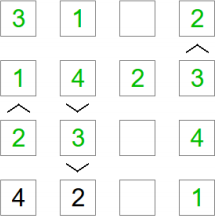
\includegraphics[width=0.3\linewidth]{futo.png}
		\caption{Przykładowa plansza Futoshiki}
		\label{fig:futoshiki_board}
	\end{figure}
	Oprócz wspomnianego już wcześniej ograniczenia nakładanego na kolumny i wiersze, w tym problemie definiuje się jeszcze jedno. Na obrazku \ref{fig:futoshiki_board} jest pokazane jako znaki nierówności pomiędzy dwoma sąsiadującymi polami. Oznacza to, że wartości przypisane tym zmiennym muszą spełniać daną nierówność. Przykład niespełnienia tego typu ograniczenia jest został przedstawiony na rysunku \ref{fig:futoshiki_board_incorrect}.
	\begin{figure}[H]
		\centering
		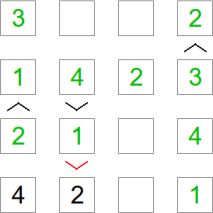
\includegraphics[width=0.3\linewidth]{futo2.png}
		\caption{Niepoprawnie uzupełniona plansza Futoshiki}
		\label{fig:futoshiki_board_incorrect}
	\end{figure}
	\subsubsection{Skyscrapper}
	Skyscrapper jest łamigłówką logiczną, w której wartości przypisywane zmiennym reprezentują wysokość wieżowca stawianego na danym polu. W tym problemie definiuje się dodatkowe ograniczenie, poza tym nakładanym na kolumny i wiersze. Na każdym z boków planszy, obok każdego pola tego boku, może być napisana liczba, mówiąca ile wieżowców powinno być widać w wierszu lub kolumnie, jeżeli spojrzeć na planszę z tego miejsca. Jeżeli wyższy budynek znajduje się przed niższym, to go zasłania. Przykładowa plansza jest przedstawiona na rysunku \ref{fig:skyscrapper_board}, a przykład niespełnienia ograniczenia na rysunku \ref{fig:skyscrapper_board_incorrect}.
	\begin{figure}[H]
		\centering
		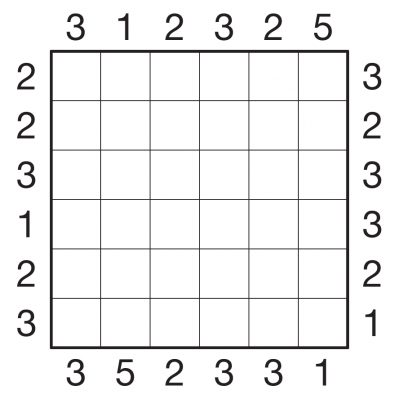
\includegraphics[width=0.3\linewidth]{skyscrapper.png}
		\caption{Przykładowa plansza do łamigłówki Skyscrapper}
		\label{fig:skyscrapper_board}
	\end{figure}
	\begin{figure}[H]
		\centering
		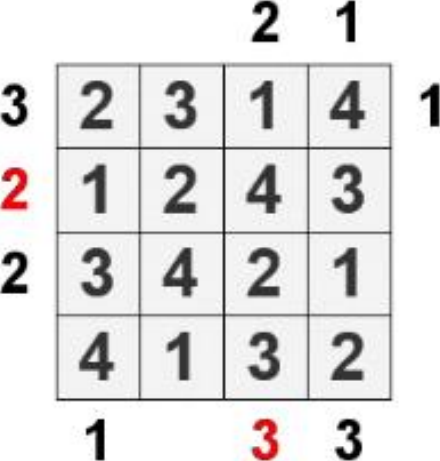
\includegraphics[width=0.3\linewidth]{skyscrapper2.png}
		\caption{Przykład niespełnienia ograniczenia w łamigłówce Skyscrapper}
		\label{fig:skyscrapper_board_incorrect}
	\end{figure}
	\subsection{Proponowane rozwiązania}
	\subsubsection{Algorytm przeszukiwania przyrostowego z powracaniem (\textit{Backtracking})}
	Algorytm ten ma na celu ograniczyć liczbę sprawdzanych rozwiązań. Wybierana jest zmienna, a następnie jest jej przypisywana wartość z dziedziny. Jeżeli po takim przypisaniu żadne ograniczenie nie zostało złamane, to algorytm przechodzi do przypisania wartości następnej zmiennej. Jeżeli w dziedzinie aktualnie rozpatrywanej zmiennej nie istnieje wartość niełamiąca żadnego z ograniczeń, następuje powrót do poprzedniej zmiennej i próba przypisania kolejnej wartości z jej dziedziny.\\
	Zadanie jest rozwiązanie w momencie kiedy wszystkie zmienne mają przypisane wartości i żadne ograniczenie nie jest złamane.
	\subsubsection{Algorytm sprawdzania w przód (\textit{Forward checking})}
	Algorytm ten postępuje podobnie do wspomnianego wcześniej. Różnica jest taka, że po każdym przypisaniu wartości do zmiennej, jeżeli ograniczenia są spełnione, to wykonywany jest dodatkowy krok. Z dziedziny wszystkich zmiennych uwikłanych w ograniczenia z aktualnie rozpatrywaną zmienną, usuwane są wartości, które powodowałyby złamanie jakiegoś ograniczenia. Jeżeli po tym procesie dziedzina którejkolwiek ze zmiennych jest pusta, to aktualnej zmiennej przypisuje się kolejną wartość z dziedziny.\\
	W znaczący sposób ogranicza to liczbę przeglądanych rozwiązań, ale procedura usuwania wartości z dziedziny zmiennych jest dość złożona, więc nie zawsze przekłada się to na zysk czasowy. 
	
	\subsubsection{Heurstyki wyboru zmiennych i wartości}\label{sub:heuristics}
	\paragraph{Wybór zmiennej do wartościowania}\mbox{}\\
	Do wyboru zmiennej do wartościowania została w tej pracy wybrana heurystyka \textit{najmniejszej liczby pozostałych wartości} (\textit{Minimum Remaining Values}). Jako następna zmienna do wartościowania wybierana będzie ta, której pozostało najmniej dostępnych wartości w dziedzinie. Heurystyka ta jest naturalnym uzupełnieniem algorytmu sprawdzania w przód. W przypadku algorytmu przeszukiwania przyrostowego z powrotami generuje ona spory narzut obliczeniowy, ponieważ wymaga wykonania obliczeń, których ten algorytm normalnie nie wykonuje.\\
	Do rozwiązywania remisów (sytuacji gdy zmienne mają taką samą liczbę dostępnych wartości) zostanie użyta heurystyka wybierająca zmienną uwikłaną w najwięcej ograniczeń. Para ta będzie w dalszej części pracy nazywana w skrócie heurystyką \textit{MRV}.\\
	Niestatyczny wybór zmiennych do wartościowania potencjalnie oferuje duży zysk, ponieważ pozwala ustawić zmienne w kolejności generującej zdecydowanie mniejsze drzewo poszukiwań.
	\paragraph{Wybór wartości dla zmiennej}\mbox{}\\
	Do wyboru następnej wartości dla zmiennej zostanie użyta heurystyka \textit{najmniej ograniczającej wartości}. Wybiera ona dla zmiennej taką wartość, która eliminuje najmniej dopuszczalnych wartości z dziedzin powiązanych zmiennych.\\
	Sformułowanie celu jako znalezienia wszystkich rozwiązań problemu, sprawia że heurystyka ta nie powinna mieć wpływu na liczbę sprawdzonych rozwiązań, ponieważ i tak należy sprawdzić wszystkie dopuszczalne wartości dla każdej ze zmiennych. Rzeczą którą można w tym przypadku badać jest czas i liczba rozwiązań sprawdzonych do momentu znalezienia pierwszego rozwiązania.
	\subsubsection{Usprawnienia wprowadzone do ograniczeń}
	Aby zmniejszyć liczbę sprawdzanych rozwiązań i potencjalnie przyspieszyć działanie algorytmów, do sposobu rozpatrywania spełnienia ograniczeń zostały wprowadzone niewielkie zmiany, wynikające wprost z ich logiki.
	\paragraph{Futoshiki}\mbox{}\\
	Ograniczenie mówiące o nierówności wartości dwóch zmiennych można by rozpatrywać dopiero w momencie przypisania obu z nich. Znając jednak pełną dziedzinę zmiennych, można wyciągnąć następujące wnioski:
	\begin{itemize}
		\item jeżeli do "mniejszej" zmiennej została przypisana największa wartość z dziedziny, to ograniczenie nie jest spełnione,
		\item jeżeli do "większej" zmiennej została przypisana najmniejsza wartość z dziedziny, to ograniczenie nie jest spełnione.
	\end{itemize}
	\paragraph{Skyscrapper}\mbox{}\\
	Ograniczenie "widzialności" wieżowców można rozszerzyć w następujący sposób:
	\begin{itemize}
		\item jeżeli do pierwszej zmiennej widzianej, z którejś ze stron została przypisana największa wartość z dziedziny, a z tej strony powinno być widać więcej niż 1 wieżowiec, to ograniczenie nie jest spełnione,
		\item jeżeli do pierwszej zmiennej widzianej, z którejś ze stron została przypisana najmniejsza wartość z dziedziny, a z tej strony powinno być widać tylko 1 wieżowiec, to ograniczenie nie jest spełnione.
	\end{itemize}

	\section{Badania}
	W sekcji badań wykorzystywane będą następujące oznaczenia:
	\begin{itemize}
		\item BT - algorytm przeszukiwania przyrostowego z powrotami (\textit{Backtracking}),
		\item FC - algorytm sprawdzania w przód (\textit{Forward checking}),
		\item MRV - wspomniana w sekcji \ref{sub:heuristics} heurystyka wyboru zmiennej do wartościowania
		\item VH - wspomniana w sekcji \ref{sub:heuristics} heurystyka wyboru wartości dla zmiennej
		\item BTM, FCM - odpowiednio algorytm BT i FC z zastosowaną heurystyką MRV
	\end{itemize}
	\subsection{Czas działania i liczba węzłów drzewa rozwiązań}
	\subsubsection{Futoshiki}
	
	\begin{table}[H]
		\caption{Liczba węzłów drzewa rozwiąząń przegladanych przez algorytmy dla różnych instancji problemu Futoshiki}
		\label{tab:solutions_futo}
		\begin{center}
			\begin{tabular}{|l|r|r|r|r|}
				\hline
				& \multicolumn{1}{c|}{\textbf{BT}} & \multicolumn{1}{c|}{\textbf{FC}} & \multicolumn{1}{c|}{\textbf{BT+MRV}} & \multicolumn{1}{c|}{\textbf{FC+MRV}} \\ \hline
				test\_futo\_4\_0 & 295                              & 125                              & 27                                   & 25                                   \\ \hline
				test\_futo\_4\_1 & 327                              & 161                              & 35                                   & 31                                   \\ \hline
				test\_futo\_4\_2 & 172                              & 80                               & 56                                   & 49                                   \\ \hline
				test\_futo\_5\_0 & 1361                             & 355                              & 59                                   & 45                                   \\ \hline
				test\_futo\_5\_1 & 4664                             & 1711                             & 87                                   & 67                                   \\ \hline
				test\_futo\_5\_2 & 352                              & 159                              & 96                                   & 82                                   \\ \hline
				test\_futo\_6\_0 & 21120                            & 3811                             & 166                                  & 142                                  \\ \hline
				test\_futo\_6\_1 & 86685                            & 23489                            & 214                                  & \textbf{187}                         \\ \hline
				test\_futo\_6\_2 & 161079                           & 56986                            & 679                                  & \textbf{532}                         \\ \hline
				test\_futo\_7\_0 & 35648494                         & 10309677                         & 52583                                & \textbf{40525}                       \\ \hline
				test\_futo\_7\_1 & 9367837                          & 529143                           & 33591                                & 24181                                \\ \hline
				test\_futo\_7\_2 & 7616386                          & 2399217                          & 40573                                & 27054                                \\ \hline
				test\_futo\_8\_0 & 3026907845                       & 1117                             & \textbf{1}                           & \textbf{1}                           \\ \hline
				test\_futo\_8\_1 & n/a                              & 458028557                        & 820475                               & \textbf{591495}                      \\ \hline
				test\_futo\_8\_2 & 77198485                         & 17540373                         & 16445380                             & 12106524                             \\ \hline
				test\_futo\_9\_0 & n/a                              & 269559                           & 35787                                & 31290                                \\ \hline
				test\_futo\_9\_1 & n/a                              & n/a                              & 6811876                              & 4977377                              \\ \hline
				test\_futo\_9\_2 & n/a                              & n/a                              & 6541040                              & 4472736                              \\ \hline
			\end{tabular}
		\end{center}
	\end{table}
	
	W tabeli \ref{tab:solutions_futo} przedstawione zostały liczby węzłów drzewa rozwiązań, odwiedzanych przez poszczególne algorytmy, dla różnych instancji problemu Futoshiki. Każdy z opisywanych algorytmów został tam przedstawiony w 2 wersjach. Jedna z nich korzystała z heurystyki MRV do wyboru zmiennej do wartościowania, a druga nie. 
	Pierwsza rzecz, która rzuca się w oczy, to dużo mniejsza liczba przeglądanych przez algorytm FC w stosunku do algorytmu BT. Bardzo ważne jest, aby zauważyć, jak dużą różnicę w liczbie przeglądanych węzłów wprowadza zastosowanie heurystyki MRV. W tabeli pogrubione zostały te miejsca, dla których zysk był największy. Najlepiej widać to najprawdopodobniej na przykładzie pliku test\_futo\_8\_0, gdzie zastosowanie tej heurystyki pozwoliło już w pierwszym kroku stwierdzić, że ten problem nie posiada rozwiązania. Drugim ciekawy przypadek widać dla pliku test\_futo\_8\_1, gdzie zysk był ponad 700-krotny.
	
	\begin{table}[H]
		\caption{Czasy przetwarzania poszczególnych algorytmów dla różnych instancji problemu Futoshiki}
		\label{tab:times_futo}
		\begin{center}
			\begin{tabular}{|l|r|r|r|r|}
				\hline
				& \multicolumn{1}{c|}{\textbf{BT (s)}} & \multicolumn{1}{c|}{\textbf{FC (s)}} & \multicolumn{1}{c|}{\textbf{BT + MRV (s)}} & \multicolumn{1}{c|}{\textbf{FC + MRV (s)}} \\ \hline
				test\_futo\_4\_0 & 0,0015                           & 0,0007                           & 0,0016                                 & 0,0139                                 \\ \hline
				test\_futo\_4\_1 & 0,0004                           & 0,0010                           & 0,0016                                 & 0,0051                                 \\ \hline
				test\_futo\_4\_2 & 0,0002                           & 0,0004                           & 0,0020                                 & 0,0072                                 \\ \hline
				test\_futo\_5\_0 & 0,0019                           & 0,0020                           & 0,0056                                 & 0,0135                                 \\ \hline
				test\_futo\_5\_1 & 0,0053                           & 0,0069                           & 0,0071                                 & 0,0049                                 \\ \hline
				test\_futo\_5\_2 & 0,0005                           & 0,0009                           & 0,0073                                 & 0,0037                                 \\ \hline
				test\_futo\_6\_0 & 0,0313                           & 0,0201                           & 0,0227                                 & 0,0117                                 \\ \hline
				test\_futo\_6\_1 & 0,1050                           & 0,1551                           & 0,0263                                 & 0,0067                                 \\ \hline
				test\_futo\_6\_2 & 0,1798                           & 0,3180                           & 0,0899                                 & 0,0961                                 \\ \hline
				test\_futo\_7\_0 & 48,5966                          & 62,1622                          & 9,9277                                 & 0,6738                                 \\ \hline
				test\_futo\_7\_1 & 12,8833                          & 4,2271                           & 6,7674                                 & 0,3085                                 \\ \hline
				test\_futo\_7\_2 & 10,3744                          & 17,0219                          & 8,6324                                 & 0,2909                                 \\ \hline
				test\_futo\_8\_0 & 4491,2230                        & 0,1625                           & 0,0010                                 & 0,0002                                 \\ \hline
				test\_futo\_8\_1 & n/a                              & 2813,9495                        & 254,7720                               & 7,7844                                 \\ \hline
				test\_futo\_8\_2 & 116,0373                         & 148,2639                         & 4830,8584                              & 154,3986                               \\ \hline
				test\_futo\_9\_0 & n/a                              & 2,1556                           & 10,8396                                & 0,3307                                 \\ \hline
				test\_futo\_9\_1 & n/a                              & n/a                              & 2657,8022                              & 63,5044                                \\ \hline
				test\_futo\_9\_2 & n/a                              & n/a                              & 2677,7288                              & 64,6978                                \\ \hline
			\end{tabular}
		\end{center}
	\end{table}

	W tabeli \ref{tab:times_futo} przedstawione zostały czasy przetwarzania dla różnych algorytmów na różnych instancjach problemu Futoshiki. Można tam zauważyć m.in. to, że gdy po zastosowaniu heurystyki MRV, udało się rozwiązać duże instancje problemów, które nie były możliwe do rozwiązania bez tego. Heurystyka ta bardzo dobrze komponuje się w działanie algorytmu FC. Dzięki temu narzut obliczeniowy nie jest tam aż tak duży i dla większych instancji problemów pozwala to znacznie przyspieszyć ich rozwiązywanie metodą sprawdzania w przód.\\
	Jeżeli chodzi o algorytm BT, to widać, że o ile zastosowanie w nim tej heurystyki czasami daje sensowne rezultaty, o tyle narzut obliczeniowy jest ogromny. Co za tym idzie, użycie jej na dużych instancjach problemów, potrafi znacząco spowolnić jego działanie.
	
	\subsubsection{Skyscrapper}
	
	\begin{table}[H]
		\caption{Liczba węzłów drzewa rozwiąząń przeglądanych przez algorytmy}
		\label{tab:skyscrapper_solutions}
		\begin{center}
			\begin{tabular}{|l|r|r|r|r|}
				\hline
				& \multicolumn{1}{c|}{\textbf{BT}} & \multicolumn{1}{c|}{\textbf{FC}} & \multicolumn{1}{c|}{\textbf{BT + MRV}} & \multicolumn{1}{c|}{\textbf{FC + MRV}} \\ \hline
				test\_sky\_4\_0 & 215                              & 115                              & 110                                    & 81                                     \\ \hline
				test\_sky\_4\_1 & 161                              & 77                               & 74                                     & 58                                     \\ \hline
				test\_sky\_4\_2 & 304                              & 139                              & 193                                    & 164                                    \\ \hline
				test\_sky\_4\_3 & 1270                             & 614                              & 393                                    & 311                                    \\ \hline
				test\_sky\_4\_4 & 137                              & 76                               & 82                                     & 68                                     \\ \hline
				test\_sky\_5\_0 & 93272                            & 28099                            & 9476                                   & 6227                                   \\ \hline
				test\_sky\_5\_1 & 58713                            & 14751                            & \textbf{1816}                          & \textbf{1168}                          \\ \hline
				test\_sky\_5\_2 & 15713                            & 6139                             & 9867                                   & 7053                                   \\ \hline
				test\_sky\_5\_3 & 48598                            & 17191                            & 6393                                   & 4455                                   \\ \hline
				test\_sky\_5\_4 & 7193                             & 2538                             & 1069                                   & 705                                    \\ \hline
				test\_sky\_6\_0 & 126773                           & 55630                            & 199669                                 & 145408                                 \\ \hline
				test\_sky\_6\_1 & 375146                           & 139577                           & 133312                                 & 98099                                  \\ \hline
				test\_sky\_6\_2 & 14703689                         & 3389857                          & \textbf{538231}                        & \textbf{402902}                        \\ \hline
				test\_sky\_6\_3 & 64137671                         & 26275623                         & 6758373                                & 4955527                                \\ \hline
				test\_sky\_6\_4 & 336873                           & 159064                           & 68576                                  & 49537                                  \\ \hline
			\end{tabular}
		\end{center}
	\end{table}

	\begin{table}[H]
		\caption{Czasy przetwarzania poszczególnych algorytmów dla różnych instancji problemu Skyscrapper}
		\label{tab:skyscrapper_times}
		\begin{center}
			\begin{tabular}{|l|r|r|r|r|}
				\hline
				& \multicolumn{1}{c|}{\textbf{BT (s)}} & \multicolumn{1}{c|}{\textbf{FC (s)}} & \multicolumn{1}{l|}{\textbf{BT + MRV (s)}} & \multicolumn{1}{l|}{\textbf{FC + MRV (s)}} \\ \hline
				test\_sky\_4\_0 & 0,0002                           & 0,0005                           & 0,0026                                 & 0,0024                                 \\ \hline
				test\_sky\_4\_1 & 0,0001                           & 0,0004                           & 0,0020                                 & 0,0009                                 \\ \hline
				test\_sky\_4\_2 & 0,0002                           & 0,0006                           & 0,0042                                 & 0,0015                                 \\ \hline
				test\_sky\_4\_3 & 0,0009                           & 0,0024                           & 0,0084                                 & 0,0026                                 \\ \hline
				test\_sky\_4\_4 & 0,0001                           & 0,0004                           & 0,0025                                 & 0,0006                                 \\ \hline
				test\_sky\_5\_0 & 0,0845                           & 0,1205                           & 0,4130                                 & 0,0492                                 \\ \hline
				test\_sky\_5\_1 & 0,0533                           & 0,0569                           & 0,0791                                 & 0,0087                                 \\ \hline
				test\_sky\_5\_2 & 0,0142                           & 0,0288                           & 0,4208                                 & 0,0523                                 \\ \hline
				test\_sky\_5\_3 & 0,0464                           & 0,0749                           & 0,2787                                 & 0,0338                                 \\ \hline
				test\_sky\_5\_4 & 0,0070                           & 0,0113                           & 0,0513                                 & 0,0058                                 \\ \hline
				test\_sky\_6\_0 & 0,1405                           & 0,7224                           & 13,7718                                & 0,9643                                 \\ \hline
				test\_sky\_6\_1 & 0,3634                           & 1,0723                           & 8,7668                                 & 0,6316                                 \\ \hline
				test\_sky\_6\_2 & 14,4541                          & 16,2330                          & 34,8568                                & 2,5252                                 \\ \hline
				test\_sky\_6\_3 & 66,6152                          & 136,4960                         & 436,4031                               & 32,3194                                \\ \hline
				test\_sky\_6\_4 & 0,3229                           & 0,8969                           & 5,5211                                 & 0,3557                                 \\ \hline
			\end{tabular}
		\end{center}
	\end{table}

	W tabelach \ref{tab:skyscrapper_solutions} i \ref{tab:skyscrapper_times} przedstawione zostały wyniki badań szybkości działania algorytmów dla instancji problemów Skyscrapper.
	Wnioski, które można z nich wyciągnąć w zasadzie nie różnią się od tych dla problemu Futoshiki. Algorytm FC przegląda zdecydowanie mniej węzłów drzewa rozwiązań. Zastosowanie heurystyki MRV, dla obu algorytmów daje znaczne obniżenie liczby odwiedzanych węzłów. Zastosowanie jej razem z algorytmem FC daje bardzo dobre zyski czasowe, ale już przy algorytmie BT, przez dodatkowe obliczenia, nie jest dobrym rozwiązaniem.

	\subsection{Wpływ heurystyki wyboru wartości}
	W tej sekcji przedstawione zostały wyniki badań wpływu zastosowania heurystyki wyboru wartości na szybkość znajdowania pierwszego rozwiązania, wyrażoną w liczbie odwiedzonych węzłów i czasie potrzebnym na jego znalezienie.\\
	Badania zostały przeprowadzone pod takim kątem, ponieważ tak jak wspomniano już wcześniej, przy zdefiniowaniu celu problemu jako znalezienia wszystkich istniejących rozwiązań, kolejność wyboru wartości nie ma żadnego wpływu na liczbę odwiedzanych przez algorytmy węzłów. Dzieje się tak, ponieważ aby znaleźć wszystkie rozwiązania, i tak należy przejrzeć wszystkie dopuszczalne w danym węźle wartości.

	\begin{table}[H]
		\caption{Liczba węzłów drzewa rozwiąząń przegladanych przez algorytmy do znalezienia pierwszego rozwiązania dla problemów Futoshiki}
		\label{tab:vh_mrv}
		\begin{center}
			\begin{tabular}{|l|r|r|r|r|}
				\hline
				& \multicolumn{1}{c|}{\textbf{BTM}} & \multicolumn{1}{l|}{\textbf{BTM + VH}} & \multicolumn{1}{c|}{\textbf{FCM}} & \multicolumn{1}{c|}{\textbf{FCM+ VH}} \\ \hline
				test\_futo\_4\_0 & 16                                     & 16                                          & 16                                     & 16                                          \\ \hline
				test\_futo\_4\_1 & 21                                     & \textbf{17}                                 & 19                                     & \textbf{17}                                 \\ \hline
				test\_futo\_4\_2 & 46                                     & 46                                          & 41                                     & 41                                          \\ \hline
				test\_futo\_5\_0 & 59                                     & \textbf{57}                                 & \textbf{45}                            & 46                                          \\ \hline
				test\_futo\_5\_1 & 78                                     & 78                                          & 63                                     & 63                                          \\ \hline
				test\_futo\_5\_2 & \textbf{29}                            & 45                                          & \textbf{27}                            & 42                                          \\ \hline
				test\_futo\_6\_0 & 160                                    & \textbf{67}                                 & 137                                    & \textbf{61}                                 \\ \hline
				test\_futo\_6\_1 & 138                                    & \textbf{132}                                & 121                                    & \textbf{116}                                \\ \hline
				test\_futo\_6\_2 & \textbf{149}                           & 317                                         & \textbf{124}                           & 260                                         \\ \hline
				test\_futo\_7\_0 & 23030                                  & \textbf{20638}                              & 18024                                  & \textbf{16180}                              \\ \hline
				test\_futo\_7\_1 & \textbf{21437}                         & 30681                                       & \textbf{15621}                         & 21186                                       \\ \hline
				test\_futo\_7\_2 & 32752                                  & \textbf{30553}                              & 21744                                  & \textbf{21335}                              \\ \hline
			\end{tabular}
		\end{center}
	\end{table}

\begin{table}[H]
	\caption{Czas przetwarzania do znalezienia pierwszego rozwiązania dla problemów Futoshiki}
	\label{tab:vh_no_mrv}
	\begin{center}
		\begin{tabular}{|l|r|r|r|r|}
			\hline
			& \multicolumn{1}{c|}{\textbf{BTM (s)}} & \multicolumn{1}{l|}{\textbf{BTM + VH (s)}} & \multicolumn{1}{c|}{\textbf{FCM (s)}} & \multicolumn{1}{c|}{\textbf{FCM + VH (s)}} \\ \hline
			test\_futo\_4\_0 & 0,0011                            & 0,0012                                 & 0,0101                            & 0,0134                                 \\ \hline
			test\_futo\_4\_1 & 0,0009                            & 0,0009                                 & 0,0028                            & 0,0032                                 \\ \hline
			test\_futo\_4\_2 & 0,0017                            & 0,0020                                 & 0,0065                            & 0,0057                                 \\ \hline
			test\_futo\_5\_0 & 0,0055                            & 0,0068                                 & 0,0134                            & 0,0085                                 \\ \hline
			test\_futo\_5\_1 & 0,0062                            & 0,0087                                 & 0,0045                            & 0,0051                                 \\ \hline
			test\_futo\_5\_2 & 0,0019                            & 0,0043                                 & 0,0009                            & 0,0081                                 \\ \hline
			test\_futo\_6\_0 & 0,0218                            & 0,0110                                 & 0,0114                            & 0,0037                                 \\ \hline
			test\_futo\_6\_1 & 0,0172                            & 0,0196                                 & 0,0048                            & 0,0064                                 \\ \hline
			test\_futo\_6\_2 & 0,0134                            & 0,0528                                 & 0,0255                            & 0,0375                                 \\ \hline
			test\_futo\_7\_0 & 4,2814                            & 5,6408                                 & 0,3443                            & 0,4907                                 \\ \hline
			test\_futo\_7\_1 & 4,1773                            & 9,4359                                 & 0,1930                            & 0,4368                                 \\ \hline
			test\_futo\_7\_2 & 6,8676                            & 9,9061                                 & 0,2321                            & 0,4498                                 \\ \hline
		\end{tabular}
	\end{center}
\end{table}

\begin{table}[H]
	\caption{Liczba węzłów drzewa rozwiąząń przegladanych przez algorytmy do znalezienia pierwszego rozwiązania dla problemów Skyscrapper}
	\label{tab:vh_sky_number}
	\begin{center}
		\begin{tabular}{|l|r|r|r|r|}
			\hline
			& \multicolumn{1}{c|}{\textbf{BTM}} & \multicolumn{1}{c|}{\textbf{BTM + VH}} & \multicolumn{1}{c|}{\textbf{FCM}} & \multicolumn{1}{c|}{\textbf{FCM + VH}} \\ \hline
			test\_sky\_6\_0 & \textbf{126192}                   & 131629                                 & \textbf{90921}                    & 95082                                  \\ \hline
			test\_sky\_6\_1 & 58130                             & \textbf{50396}                         & 43637                             & \textbf{37344}                         \\ \hline
			test\_sky\_6\_2 & \textbf{202190}                   & 211993                                 & \textbf{151972}                   & 160707                                 \\ \hline
			test\_sky\_6\_3 & \textbf{6279151}                  & 6329223                                & 4606340                           & \textbf{4601170}                       \\ \hline
			test\_sky\_6\_4 & \textbf{52059}                    & 54246                                  & \textbf{37588}                    & 38667                                  \\ \hline
		\end{tabular}
	\end{center}
\end{table}

\begin{table}[H]
	\caption{Czasy przetwarzania do znalezienia pierwszego rozwiązania dla problemów Skyscrapper}
	\label{tab:vh_sky_times}
	\begin{center}
		\begin{tabular}{|l|r|r|r|r|}
			\hline
			& \multicolumn{1}{c|}{\textbf{BTM (s)}} & \multicolumn{1}{c|}{\textbf{BTM + VH (s)}} & \multicolumn{1}{c|}{\textbf{FCM (s)}} & \multicolumn{1}{c|}{\textbf{FCM + VH (s)}} \\ \hline
			test\_sky\_6\_0 & 8,7182                           & 12,4947                             & 0,6015                       & 1,3103                             \\ \hline
			test\_sky\_6\_1 & 3,8109                        & 4,9899                              & 0,2768                       & 0,4737                             \\ \hline
			test\_sky\_6\_2 & 12,7111                        & 18,6572                              & 0,9401                        & 1,9689                             \\ \hline
			test\_sky\_6\_3 & 405,1843                        & 806,1923                               & 30,0207                        & 59,8440                              \\ \hline
			test\_sky\_6\_4 & 4,1970                        & 6,1803                              & 0,2709                       & 0,5504                            \\ \hline
		\end{tabular}
	\end{center}
\end{table}
Jak widać we wszystkich tabelach przedstawionych powyżej, skutki zastosowania heurystyki wyboru wartości dla zmiennej nie są tak proste do przewidzenia jak tej odpowiedzialnej za wybór zmiennej. W wynikach widać, że zastosowanie heurystyki potrafi poprawić szybkość znajdowania pierwszego rozwiązania, jak i ją pogorszyć. Zdaje się to być cecha poszczególnych instancji problemu, bardziej niż samej heurystyki.

\section{Profilowanie kodu}
Aby wyszukać potencjalne problemy w implementacji i usprawnić działanie programu, przeprowadzone zostało profilowanie kodu pod kątem użycia czasu procesora przez poszczególne fragmenty programu.
\begin{figure}[H]
	\centering
	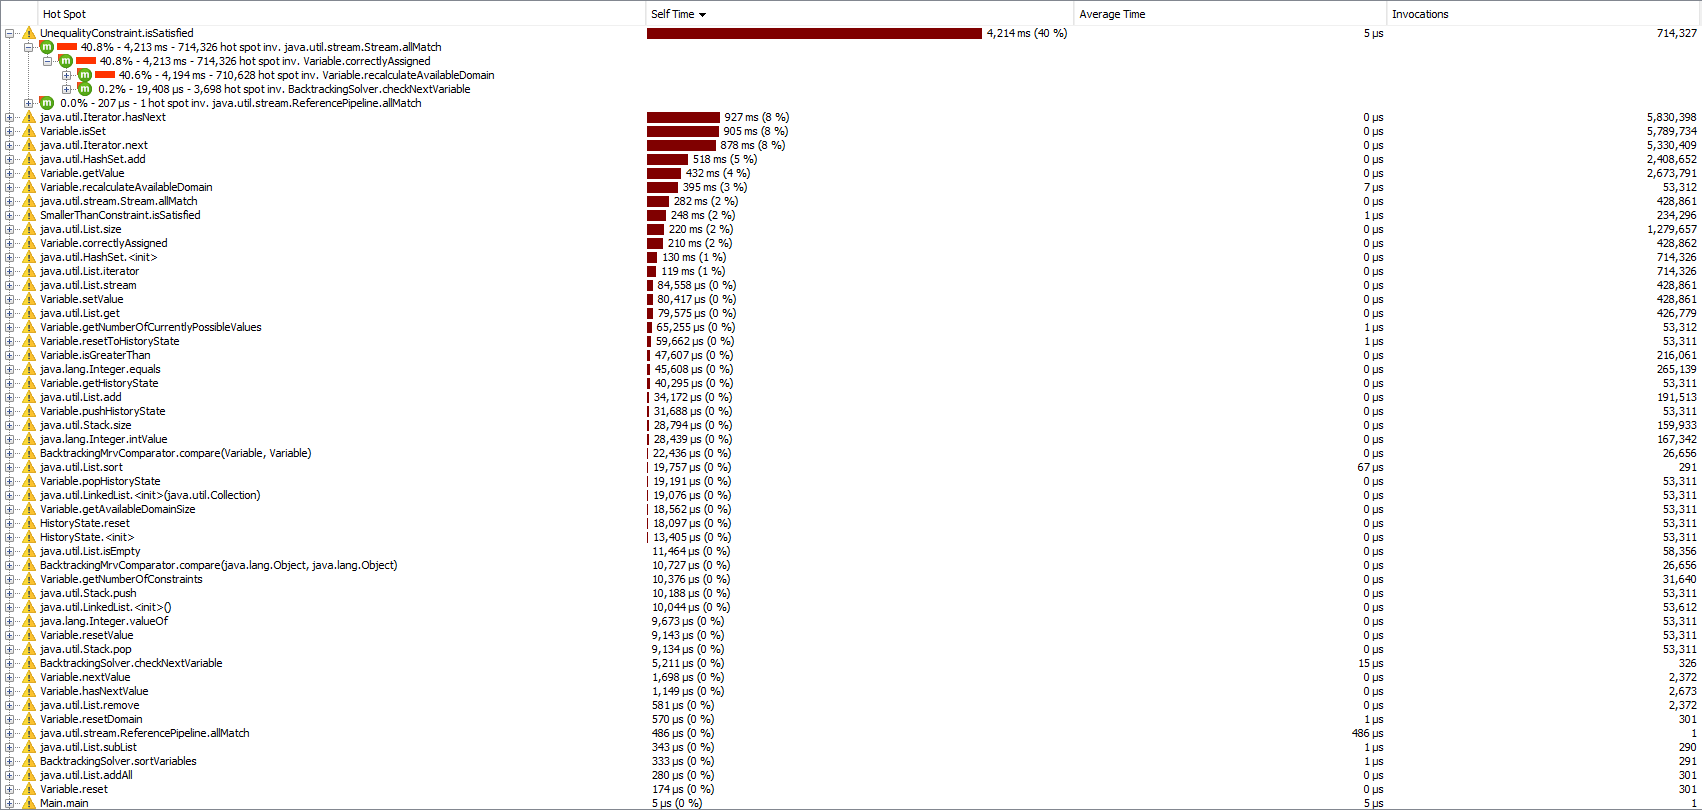
\includegraphics[width=1\linewidth]{bt_futo_mrv.png}
	\caption{Okno profilera przy uruchomionym algorytmie BT z heurystyką MRV}
	\label{fig:bt_mrv_profiling}
\end{figure}

\begin{figure}[H]
	\centering
	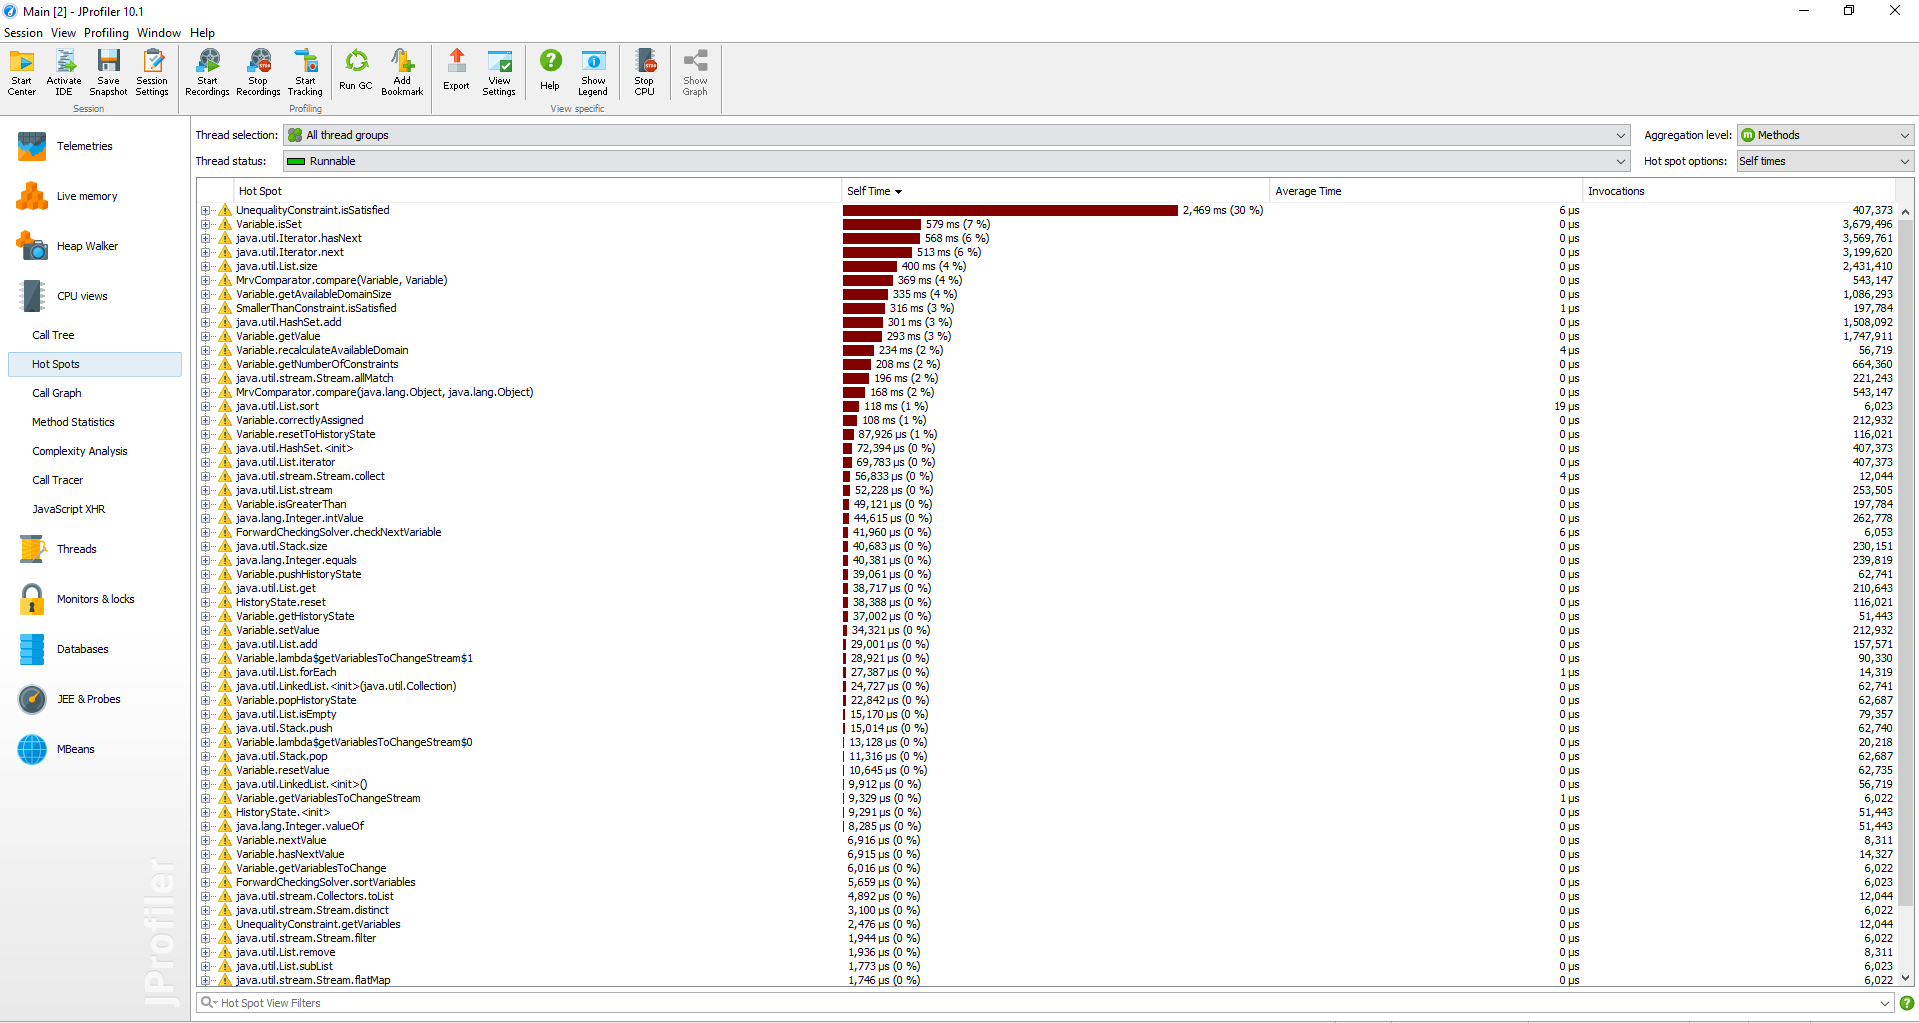
\includegraphics[width=1\linewidth]{fc_futo.png}
	\caption{Okno profilera przy uruchomionym algorytmie FC}
	\label{fig:fc_futo_profiling}
\end{figure}

Z przeprowadzonej analizy wynikło, że najczęściej używanym fragmentem kodu, niezależnie od uruchamianego algorytmu jest metoda UnequalityConstraint.isSatisfied(), więc tam właśnie został położony nacisk na optymalizację.

\section{Wnioski}
Problemy spełniania ograniczeń, przez swoją bardzo szybko rosnącą przestrzeń rozwiązań stanowią spore wyzwanie obliczeniowe. Algorytmy przeszukiwania przyrostowego z powracaniem i sprawdzania w przód, oferują efektywny sposób przeszukiwania tej przestrzeni dla dowolnego problemu sforumułowanego w terminach zmiennych i ograniczeń. Podsumowując, oba zbadane algorytmy wraz z przebadanymi heurystykami, stanowią bardzo dobre, ogólne narzędzia do rozwiązywania złożonych problemów spełniania ograniczeń. Końcowo jednak ze wszystkich zbadanych kombinacji, algorytm sprawdzania w przód z dodatkowym zastosowaniem heurystyki do wyboru zmiennej, wydaje się być najlepszym rozwiązaniem do dużych instancji tego typu problemów. 
\end{document}